\documentclass[twoside]{book}

% Packages required by doxygen
\usepackage{fixltx2e}
\usepackage{calc}
\usepackage{doxygen}
\usepackage[export]{adjustbox} % also loads graphicx
\usepackage{graphicx}
\usepackage[utf8]{inputenc}
\usepackage{makeidx}
\usepackage{multicol}
\usepackage{multirow}
\PassOptionsToPackage{warn}{textcomp}
\usepackage{textcomp}
\usepackage[nointegrals]{wasysym}
\usepackage[table]{xcolor}

% Font selection
\usepackage[T1]{fontenc}
\usepackage[scaled=.90]{helvet}
\usepackage{courier}
\usepackage{amssymb}
\usepackage{sectsty}
\renewcommand{\familydefault}{\sfdefault}
\allsectionsfont{%
  \fontseries{bc}\selectfont%
  \color{darkgray}%
}
\renewcommand{\DoxyLabelFont}{%
  \fontseries{bc}\selectfont%
  \color{darkgray}%
}
\newcommand{\+}{\discretionary{\mbox{\scriptsize$\hookleftarrow$}}{}{}}

% Page & text layout
\usepackage{geometry}
\geometry{%
  a4paper,%
  top=2.5cm,%
  bottom=2.5cm,%
  left=2.5cm,%
  right=2.5cm%
}
\tolerance=750
\hfuzz=15pt
\hbadness=750
\setlength{\emergencystretch}{15pt}
\setlength{\parindent}{0cm}
\setlength{\parskip}{3ex plus 2ex minus 2ex}
\makeatletter
\renewcommand{\paragraph}{%
  \@startsection{paragraph}{4}{0ex}{-1.0ex}{1.0ex}{%
    \normalfont\normalsize\bfseries\SS@parafont%
  }%
}
\renewcommand{\subparagraph}{%
  \@startsection{subparagraph}{5}{0ex}{-1.0ex}{1.0ex}{%
    \normalfont\normalsize\bfseries\SS@subparafont%
  }%
}
\makeatother

% Headers & footers
\usepackage{fancyhdr}
\pagestyle{fancyplain}
\fancyhead[LE]{\fancyplain{}{\bfseries\thepage}}
\fancyhead[CE]{\fancyplain{}{}}
\fancyhead[RE]{\fancyplain{}{\bfseries\leftmark}}
\fancyhead[LO]{\fancyplain{}{\bfseries\rightmark}}
\fancyhead[CO]{\fancyplain{}{}}
\fancyhead[RO]{\fancyplain{}{\bfseries\thepage}}
\fancyfoot[LE]{\fancyplain{}{}}
\fancyfoot[CE]{\fancyplain{}{}}
\fancyfoot[RE]{\fancyplain{}{\bfseries\scriptsize Generated by Doxygen }}
\fancyfoot[LO]{\fancyplain{}{\bfseries\scriptsize Generated by Doxygen }}
\fancyfoot[CO]{\fancyplain{}{}}
\fancyfoot[RO]{\fancyplain{}{}}
\renewcommand{\footrulewidth}{0.4pt}
\renewcommand{\chaptermark}[1]{%
  \markboth{#1}{}%
}
\renewcommand{\sectionmark}[1]{%
  \markright{\thesection\ #1}%
}

% Indices & bibliography
\usepackage{natbib}
\usepackage[titles]{tocloft}
\setcounter{tocdepth}{3}
\setcounter{secnumdepth}{5}
\makeindex

% Hyperlinks (required, but should be loaded last)
\usepackage{ifpdf}
\ifpdf
  \usepackage[pdftex,pagebackref=true]{hyperref}
\else
  \usepackage[ps2pdf,pagebackref=true]{hyperref}
\fi
\hypersetup{%
  colorlinks=true,%
  linkcolor=blue,%
  citecolor=blue,%
  unicode%
}

% Custom commands
\newcommand{\clearemptydoublepage}{%
  \newpage{\pagestyle{empty}\cleardoublepage}%
}

\usepackage{caption}
\captionsetup{labelsep=space,justification=centering,font={bf},singlelinecheck=off,skip=4pt,position=top}

%===== C O N T E N T S =====

\begin{document}

% Titlepage & ToC
\hypersetup{pageanchor=false,
             bookmarksnumbered=true,
             pdfencoding=unicode
            }
\pagenumbering{alph}
\begin{titlepage}
\vspace*{7cm}
\begin{center}%
{\Large Vector }\\
\vspace*{1cm}
{\large Generated by Doxygen 1.8.13}\\
\end{center}
\end{titlepage}
\clearemptydoublepage
\pagenumbering{roman}
\tableofcontents
\clearemptydoublepage
\pagenumbering{arabic}
\hypersetup{pageanchor=true}

%--- Begin generated contents ---
\chapter{Hierarchical Index}
\section{Class Hierarchy}
This inheritance list is sorted roughly, but not completely, alphabetically\+:\begin{DoxyCompactList}
\item Action\+Listener\begin{DoxyCompactList}
\item \contentsline{section}{Window}{\pageref{class_window}}{}
\end{DoxyCompactList}
\item \contentsline{section}{Double\+Point}{\pageref{class_double_point}}{}
\item J\+Frame\begin{DoxyCompactList}
\item \contentsline{section}{Window}{\pageref{class_window}}{}
\end{DoxyCompactList}
\item \contentsline{section}{Shape}{\pageref{class_shape}}{}
\item \contentsline{section}{Utils}{\pageref{class_utils}}{}
\item \contentsline{section}{Vector}{\pageref{class_vector}}{}
\item File\+Filter\begin{DoxyCompactList}
\item \contentsline{section}{Vector\+Filter}{\pageref{class_vector_filter}}{}
\end{DoxyCompactList}
\end{DoxyCompactList}

\chapter{Class Index}
\section{Class List}
Here are the classes, structs, unions and interfaces with brief descriptions\+:\begin{DoxyCompactList}
\item\contentsline{section}{\hyperlink{class_double_point}{Double\+Point} }{\pageref{class_double_point}}{}
\item\contentsline{section}{\hyperlink{class_shape}{Shape} }{\pageref{class_shape}}{}
\item\contentsline{section}{\hyperlink{class_utils}{Utils} }{\pageref{class_utils}}{}
\item\contentsline{section}{\hyperlink{class_vector}{Vector} }{\pageref{class_vector}}{}
\item\contentsline{section}{\hyperlink{class_vector_filter}{Vector\+Filter} }{\pageref{class_vector_filter}}{}
\item\contentsline{section}{\hyperlink{class_window}{Window} }{\pageref{class_window}}{}
\end{DoxyCompactList}

\chapter{Class Documentation}
\hypertarget{class_double_point}{}\section{Double\+Point Class Reference}
\label{class_double_point}\index{Double\+Point@{Double\+Point}}
\subsection*{Public Member Functions}
\begin{DoxyCompactItemize}
\item 
double \hyperlink{class_double_point_ac077fc9eadd03e6f7caeec37265b4d08}{getX} ()
\item 
double \hyperlink{class_double_point_a23bfa07d4c1af558eb85ec06155e2740}{getY} ()
\item 
void \hyperlink{class_double_point_abf7ded4d23fddd292e089f02dae94566}{set\+Location} (double x, double y)
\item 
void \hyperlink{class_double_point_a3f02b79ca4952156c087404cf85aee7d}{translate} (double dx, double dy)
\end{DoxyCompactItemize}


\subsection{Detailed Description}
Simple implementation of Point class using double coordinates. \begin{DoxyAuthor}{Author}
Maciej Stosio 
\end{DoxyAuthor}
\begin{DoxyVersion}{Version}
1.\+0 
\end{DoxyVersion}


\subsection{Member Function Documentation}
\mbox{\Hypertarget{class_double_point_ac077fc9eadd03e6f7caeec37265b4d08}\label{class_double_point_ac077fc9eadd03e6f7caeec37265b4d08}} 
\index{Double\+Point@{Double\+Point}!getX@{getX}}
\index{getX@{getX}!Double\+Point@{Double\+Point}}
\subsubsection{\texorpdfstring{get\+X()}{getX()}}
{\footnotesize\ttfamily double Double\+Point.\+getX (\begin{DoxyParamCaption}{ }\end{DoxyParamCaption})}

\begin{DoxyReturn}{Returns}
x coordinate 
\end{DoxyReturn}
\mbox{\Hypertarget{class_double_point_a23bfa07d4c1af558eb85ec06155e2740}\label{class_double_point_a23bfa07d4c1af558eb85ec06155e2740}} 
\index{Double\+Point@{Double\+Point}!getY@{getY}}
\index{getY@{getY}!Double\+Point@{Double\+Point}}
\subsubsection{\texorpdfstring{get\+Y()}{getY()}}
{\footnotesize\ttfamily double Double\+Point.\+getY (\begin{DoxyParamCaption}{ }\end{DoxyParamCaption})}

\begin{DoxyReturn}{Returns}
y coordinate 
\end{DoxyReturn}
\mbox{\Hypertarget{class_double_point_abf7ded4d23fddd292e089f02dae94566}\label{class_double_point_abf7ded4d23fddd292e089f02dae94566}} 
\index{Double\+Point@{Double\+Point}!set\+Location@{set\+Location}}
\index{set\+Location@{set\+Location}!Double\+Point@{Double\+Point}}
\subsubsection{\texorpdfstring{set\+Location()}{setLocation()}}
{\footnotesize\ttfamily void Double\+Point.\+set\+Location (\begin{DoxyParamCaption}\item[{double}]{x,  }\item[{double}]{y }\end{DoxyParamCaption})}

Change location of point 
\begin{DoxyParams}{Parameters}
{\em x} & coordinate, double type \\
\hline
{\em y} & coordinate, double type \\
\hline
\end{DoxyParams}
\mbox{\Hypertarget{class_double_point_a3f02b79ca4952156c087404cf85aee7d}\label{class_double_point_a3f02b79ca4952156c087404cf85aee7d}} 
\index{Double\+Point@{Double\+Point}!translate@{translate}}
\index{translate@{translate}!Double\+Point@{Double\+Point}}
\subsubsection{\texorpdfstring{translate()}{translate()}}
{\footnotesize\ttfamily void Double\+Point.\+translate (\begin{DoxyParamCaption}\item[{double}]{dx,  }\item[{double}]{dy }\end{DoxyParamCaption})}

Move point with vector \mbox{[}x,y\mbox{]} 
\begin{DoxyParams}{Parameters}
{\em dx} & x coordinate, double type \\
\hline
{\em dy} & y coordinate, double type \\
\hline
\end{DoxyParams}


The documentation for this class was generated from the following file\+:\begin{DoxyCompactItemize}
\item 
Double\+Point.\+java\end{DoxyCompactItemize}

\hypertarget{class_shape}{}\section{Shape Class Reference}
\label{class_shape}\index{Shape@{Shape}}


Inherited by Circle, Polygon, and Rectangle.

\subsection*{Public Member Functions}
\begin{DoxyCompactItemize}
\item 
\hyperlink{class_shape_a3d76b5d801383515923d2f9f800d0d6c}{Shape} ()
\item 
\hyperlink{class_shape_a077daea39f5e67150f6ca1b89b6fc6fd}{Shape} (Array\+List$<$ \hyperlink{class_double_point}{Double\+Point} $>$ p)
\item 
void \hyperlink{class_shape_a32626b5ccab1d89c6724af95121dc125}{add} (double x, double y)
\item 
boolean \hyperlink{class_shape_aa1c3adc5bee37da4d5972965caaec344}{is\+Selected} ()
\item 
void \hyperlink{class_shape_afa9a615b704d91064260ea688dd625f5}{select} ()
\item 
void \hyperlink{class_shape_a5fda5181466313db27d010bbf7bb50a4}{unselect} ()
\item 
void \hyperlink{class_shape_a49e29c1da103be18d279993034de99c6}{set\+Color} (Color c)
\item 
Color \hyperlink{class_shape_a4271dba03c30547a4e0c87418cc07bf8}{get\+Color} ()
\item 
Array\+List$<$ \hyperlink{class_double_point}{Double\+Point} $>$ \hyperlink{class_shape_acced47c85afcddf20b66f1820b86584a}{get\+Points} ()
\item 
abstract boolean \hyperlink{class_shape_a8b64c43dfba956f5586336c460735e1d}{valid} ()
\item 
abstract boolean \hyperlink{class_shape_ada4e95f3d5340e22d9f51db227b16daa}{include} (int x, int y)
\item 
abstract void \hyperlink{class_shape_a2b1385526d1687f2bf2c382aab40cef4}{init} ()
\item 
abstract void \hyperlink{class_shape_a2416754be161196c88e0fa1816e08c0c}{resize} (int n)
\item 
abstract void \hyperlink{class_shape_ac6c07cfa25f740b78af1c212d111fb1e}{move} (int deltaX, int deltaY)
\item 
abstract void \hyperlink{class_shape_a49dd492d72e51ebff5323f12061b970e}{draw} (Graphics2D g2d)
\item 
abstract void \hyperlink{class_shape_aeb76c0ca3c4e20d02d172ba4ce83bd2d}{preview} (Graphics2D g2d, int x, int y)
\end{DoxyCompactItemize}


\subsection{Detailed Description}
Abstract class shape and subclasses defining shapes. \begin{DoxyAuthor}{Author}
Maciej Stosio 
\end{DoxyAuthor}
\begin{DoxyVersion}{Version}
1.\+0 
\end{DoxyVersion}


\subsection{Constructor \& Destructor Documentation}
\mbox{\Hypertarget{class_shape_a3d76b5d801383515923d2f9f800d0d6c}\label{class_shape_a3d76b5d801383515923d2f9f800d0d6c}} 
\index{Shape@{Shape}!Shape@{Shape}}
\index{Shape@{Shape}!Shape@{Shape}}
\subsubsection{\texorpdfstring{Shape()}{Shape()}\hspace{0.1cm}{\footnotesize\ttfamily [1/2]}}
{\footnotesize\ttfamily Shape.\+Shape (\begin{DoxyParamCaption}{ }\end{DoxyParamCaption})}

Create shape without any points. \mbox{\Hypertarget{class_shape_a077daea39f5e67150f6ca1b89b6fc6fd}\label{class_shape_a077daea39f5e67150f6ca1b89b6fc6fd}} 
\index{Shape@{Shape}!Shape@{Shape}}
\index{Shape@{Shape}!Shape@{Shape}}
\subsubsection{\texorpdfstring{Shape()}{Shape()}\hspace{0.1cm}{\footnotesize\ttfamily [2/2]}}
{\footnotesize\ttfamily Shape.\+Shape (\begin{DoxyParamCaption}\item[{Array\+List$<$ \hyperlink{class_double_point}{Double\+Point} $>$}]{p }\end{DoxyParamCaption})}

Create new shape based on given points. 
\begin{DoxyParams}{Parameters}
{\em p} & list of \hyperlink{class_double_point}{Double\+Point}\textquotesingle{}s \\
\hline
\end{DoxyParams}


\subsection{Member Function Documentation}
\mbox{\Hypertarget{class_shape_a32626b5ccab1d89c6724af95121dc125}\label{class_shape_a32626b5ccab1d89c6724af95121dc125}} 
\index{Shape@{Shape}!add@{add}}
\index{add@{add}!Shape@{Shape}}
\subsubsection{\texorpdfstring{add()}{add()}}
{\footnotesize\ttfamily void Shape.\+add (\begin{DoxyParamCaption}\item[{double}]{x,  }\item[{double}]{y }\end{DoxyParamCaption})}

Create shape without any points. 
\begin{DoxyParams}{Parameters}
{\em x} & double number of x coordinate \\
\hline
{\em y} & double number of y coordinate \\
\hline
\end{DoxyParams}
\mbox{\Hypertarget{class_shape_a49dd492d72e51ebff5323f12061b970e}\label{class_shape_a49dd492d72e51ebff5323f12061b970e}} 
\index{Shape@{Shape}!draw@{draw}}
\index{draw@{draw}!Shape@{Shape}}
\subsubsection{\texorpdfstring{draw()}{draw()}}
{\footnotesize\ttfamily abstract void Shape.\+draw (\begin{DoxyParamCaption}\item[{Graphics2D}]{g2d }\end{DoxyParamCaption})\hspace{0.3cm}{\ttfamily [abstract]}}

Draw shape on given canvas 
\begin{DoxyParams}{Parameters}
{\em g2d} & Graphics2D context \\
\hline
\end{DoxyParams}
\mbox{\Hypertarget{class_shape_a4271dba03c30547a4e0c87418cc07bf8}\label{class_shape_a4271dba03c30547a4e0c87418cc07bf8}} 
\index{Shape@{Shape}!get\+Color@{get\+Color}}
\index{get\+Color@{get\+Color}!Shape@{Shape}}
\subsubsection{\texorpdfstring{get\+Color()}{getColor()}}
{\footnotesize\ttfamily Color Shape.\+get\+Color (\begin{DoxyParamCaption}{ }\end{DoxyParamCaption})}

Get color of shape. \begin{DoxyReturn}{Returns}
instance of Color class 
\end{DoxyReturn}
\mbox{\Hypertarget{class_shape_acced47c85afcddf20b66f1820b86584a}\label{class_shape_acced47c85afcddf20b66f1820b86584a}} 
\index{Shape@{Shape}!get\+Points@{get\+Points}}
\index{get\+Points@{get\+Points}!Shape@{Shape}}
\subsubsection{\texorpdfstring{get\+Points()}{getPoints()}}
{\footnotesize\ttfamily Array\+List$<$\hyperlink{class_double_point}{Double\+Point}$>$ Shape.\+get\+Points (\begin{DoxyParamCaption}{ }\end{DoxyParamCaption})}

Get all points in shape \begin{DoxyReturn}{Returns}
list of \hyperlink{class_double_point}{Double\+Point} 
\end{DoxyReturn}
\mbox{\Hypertarget{class_shape_ada4e95f3d5340e22d9f51db227b16daa}\label{class_shape_ada4e95f3d5340e22d9f51db227b16daa}} 
\index{Shape@{Shape}!include@{include}}
\index{include@{include}!Shape@{Shape}}
\subsubsection{\texorpdfstring{include()}{include()}}
{\footnotesize\ttfamily abstract boolean Shape.\+include (\begin{DoxyParamCaption}\item[{int}]{x,  }\item[{int}]{y }\end{DoxyParamCaption})\hspace{0.3cm}{\ttfamily [abstract]}}

Check if given point is inside the shape. 
\begin{DoxyParams}{Parameters}
{\em x} & x coordinate as integer \\
\hline
{\em y} & y coordinate as integer \\
\hline
\end{DoxyParams}
\begin{DoxyReturn}{Returns}
True if it\textquotesingle{}s inside, false if it\textquotesingle{}s not 
\end{DoxyReturn}
\mbox{\Hypertarget{class_shape_a2b1385526d1687f2bf2c382aab40cef4}\label{class_shape_a2b1385526d1687f2bf2c382aab40cef4}} 
\index{Shape@{Shape}!init@{init}}
\index{init@{init}!Shape@{Shape}}
\subsubsection{\texorpdfstring{init()}{init()}}
{\footnotesize\ttfamily abstract void Shape.\+init (\begin{DoxyParamCaption}{ }\end{DoxyParamCaption})\hspace{0.3cm}{\ttfamily [abstract]}}

Init shape -\/ generate information like width, height, radius. \mbox{\Hypertarget{class_shape_aa1c3adc5bee37da4d5972965caaec344}\label{class_shape_aa1c3adc5bee37da4d5972965caaec344}} 
\index{Shape@{Shape}!is\+Selected@{is\+Selected}}
\index{is\+Selected@{is\+Selected}!Shape@{Shape}}
\subsubsection{\texorpdfstring{is\+Selected()}{isSelected()}}
{\footnotesize\ttfamily boolean Shape.\+is\+Selected (\begin{DoxyParamCaption}{ }\end{DoxyParamCaption})}

Return wheter shape is selected or not. \begin{DoxyReturn}{Returns}
boolean 
\end{DoxyReturn}
\mbox{\Hypertarget{class_shape_ac6c07cfa25f740b78af1c212d111fb1e}\label{class_shape_ac6c07cfa25f740b78af1c212d111fb1e}} 
\index{Shape@{Shape}!move@{move}}
\index{move@{move}!Shape@{Shape}}
\subsubsection{\texorpdfstring{move()}{move()}}
{\footnotesize\ttfamily abstract void Shape.\+move (\begin{DoxyParamCaption}\item[{int}]{deltaX,  }\item[{int}]{deltaY }\end{DoxyParamCaption})\hspace{0.3cm}{\ttfamily [abstract]}}

Translate shape of vector \mbox{[}x,y\mbox{]}. 
\begin{DoxyParams}{Parameters}
{\em deltaX} & x vector value as integer \\
\hline
{\em deltaY} & y vector value as integer \\
\hline
\end{DoxyParams}
\mbox{\Hypertarget{class_shape_aeb76c0ca3c4e20d02d172ba4ce83bd2d}\label{class_shape_aeb76c0ca3c4e20d02d172ba4ce83bd2d}} 
\index{Shape@{Shape}!preview@{preview}}
\index{preview@{preview}!Shape@{Shape}}
\subsubsection{\texorpdfstring{preview()}{preview()}}
{\footnotesize\ttfamily abstract void Shape.\+preview (\begin{DoxyParamCaption}\item[{Graphics2D}]{g2d,  }\item[{int}]{x,  }\item[{int}]{y }\end{DoxyParamCaption})\hspace{0.3cm}{\ttfamily [abstract]}}

Preview shape based on given points and another, temporary point. 
\begin{DoxyParams}{Parameters}
{\em g2d} & Graphics2D context \\
\hline
{\em x} & x coordinate of temporary point as integer \\
\hline
{\em y} & y coordinate of temporary point as integer \\
\hline
\end{DoxyParams}
\mbox{\Hypertarget{class_shape_a2416754be161196c88e0fa1816e08c0c}\label{class_shape_a2416754be161196c88e0fa1816e08c0c}} 
\index{Shape@{Shape}!resize@{resize}}
\index{resize@{resize}!Shape@{Shape}}
\subsubsection{\texorpdfstring{resize()}{resize()}}
{\footnotesize\ttfamily abstract void Shape.\+resize (\begin{DoxyParamCaption}\item[{int}]{n }\end{DoxyParamCaption})\hspace{0.3cm}{\ttfamily [abstract]}}

Scal shape of n unit\textquotesingle{}s 
\begin{DoxyParams}{Parameters}
{\em n} & unit\textquotesingle{}s as integer \\
\hline
\end{DoxyParams}
\mbox{\Hypertarget{class_shape_afa9a615b704d91064260ea688dd625f5}\label{class_shape_afa9a615b704d91064260ea688dd625f5}} 
\index{Shape@{Shape}!select@{select}}
\index{select@{select}!Shape@{Shape}}
\subsubsection{\texorpdfstring{select()}{select()}}
{\footnotesize\ttfamily void Shape.\+select (\begin{DoxyParamCaption}{ }\end{DoxyParamCaption})}

Select the shape. \mbox{\Hypertarget{class_shape_a49e29c1da103be18d279993034de99c6}\label{class_shape_a49e29c1da103be18d279993034de99c6}} 
\index{Shape@{Shape}!set\+Color@{set\+Color}}
\index{set\+Color@{set\+Color}!Shape@{Shape}}
\subsubsection{\texorpdfstring{set\+Color()}{setColor()}}
{\footnotesize\ttfamily void Shape.\+set\+Color (\begin{DoxyParamCaption}\item[{Color}]{c }\end{DoxyParamCaption})}

Set color of shape. 
\begin{DoxyParams}{Parameters}
{\em c} & instance of Color class \\
\hline
\end{DoxyParams}
\mbox{\Hypertarget{class_shape_a5fda5181466313db27d010bbf7bb50a4}\label{class_shape_a5fda5181466313db27d010bbf7bb50a4}} 
\index{Shape@{Shape}!unselect@{unselect}}
\index{unselect@{unselect}!Shape@{Shape}}
\subsubsection{\texorpdfstring{unselect()}{unselect()}}
{\footnotesize\ttfamily void Shape.\+unselect (\begin{DoxyParamCaption}{ }\end{DoxyParamCaption})}

Unselect the shape. \mbox{\Hypertarget{class_shape_a8b64c43dfba956f5586336c460735e1d}\label{class_shape_a8b64c43dfba956f5586336c460735e1d}} 
\index{Shape@{Shape}!valid@{valid}}
\index{valid@{valid}!Shape@{Shape}}
\subsubsection{\texorpdfstring{valid()}{valid()}}
{\footnotesize\ttfamily abstract boolean Shape.\+valid (\begin{DoxyParamCaption}{ }\end{DoxyParamCaption})\hspace{0.3cm}{\ttfamily [abstract]}}

Check if shape is valid i.\+e. height can\textquotesingle{}t be 0. \begin{DoxyReturn}{Returns}
True if it\textquotesingle{}s valid, false if it\textquotesingle{}s not 
\end{DoxyReturn}


The documentation for this class was generated from the following file\+:\begin{DoxyCompactItemize}
\item 
Shape.\+java\end{DoxyCompactItemize}

\hypertarget{class_utils}{}\section{Utils Class Reference}
\label{class_utils}\index{Utils@{Utils}}
\subsection*{Static Public Member Functions}
\begin{DoxyCompactItemize}
\item 
\mbox{\Hypertarget{class_utils_a80584b7ec64ec0233d7c6f1846cd94a5}\label{class_utils_a80584b7ec64ec0233d7c6f1846cd94a5}} 
static String {\bfseries get\+Extension} (File f)
\end{DoxyCompactItemize}
\subsection*{Static Public Attributes}
\begin{DoxyCompactItemize}
\item 
\mbox{\Hypertarget{class_utils_ac9fd6f8e1bccc37a6cd3863c0d17201b}\label{class_utils_ac9fd6f8e1bccc37a6cd3863c0d17201b}} 
static final String {\bfseries vector} = \char`\"{}vector\char`\"{}
\end{DoxyCompactItemize}


\subsection{Detailed Description}
Util class for filter formats \begin{DoxyAuthor}{Author}
Maciej Stosio 
\end{DoxyAuthor}
\begin{DoxyVersion}{Version}
1.\+0 
\end{DoxyVersion}


The documentation for this class was generated from the following file\+:\begin{DoxyCompactItemize}
\item 
Utils.\+java\end{DoxyCompactItemize}

\hypertarget{class_vector}{}\section{Vector Class Reference}
\label{class_vector}\index{Vector@{Vector}}
\subsection*{Static Public Member Functions}
\begin{DoxyCompactItemize}
\item 
static void \hyperlink{class_vector_a8cc70560a28244131498b54747e34e96}{main} (String\mbox{[}$\,$\mbox{]} args)
\end{DoxyCompactItemize}


\subsection{Detailed Description}
Simple graphics editor. You can draw rectangles, circles and polygons then select and edit them. \begin{DoxyAuthor}{Author}
Maciej Stosio 
\end{DoxyAuthor}
\begin{DoxyVersion}{Version}
1.\+0 
\end{DoxyVersion}


\subsection{Member Function Documentation}
\mbox{\Hypertarget{class_vector_a8cc70560a28244131498b54747e34e96}\label{class_vector_a8cc70560a28244131498b54747e34e96}} 
\index{Vector@{Vector}!main@{main}}
\index{main@{main}!Vector@{Vector}}
\subsubsection{\texorpdfstring{main()}{main()}}
{\footnotesize\ttfamily static void Vector.\+main (\begin{DoxyParamCaption}\item[{String \mbox{[}$\,$\mbox{]}}]{args }\end{DoxyParamCaption})\hspace{0.3cm}{\ttfamily [static]}}

Lunch the main window. 
\begin{DoxyParams}{Parameters}
{\em args} & String\mbox{[}\mbox{]} \\
\hline
\end{DoxyParams}


The documentation for this class was generated from the following file\+:\begin{DoxyCompactItemize}
\item 
Vector.\+java\end{DoxyCompactItemize}

\hypertarget{class_vector_filter}{}\section{Vector\+Filter Class Reference}
\label{class_vector_filter}\index{Vector\+Filter@{Vector\+Filter}}
Inheritance diagram for Vector\+Filter\+:\begin{figure}[H]
\begin{center}
\leavevmode
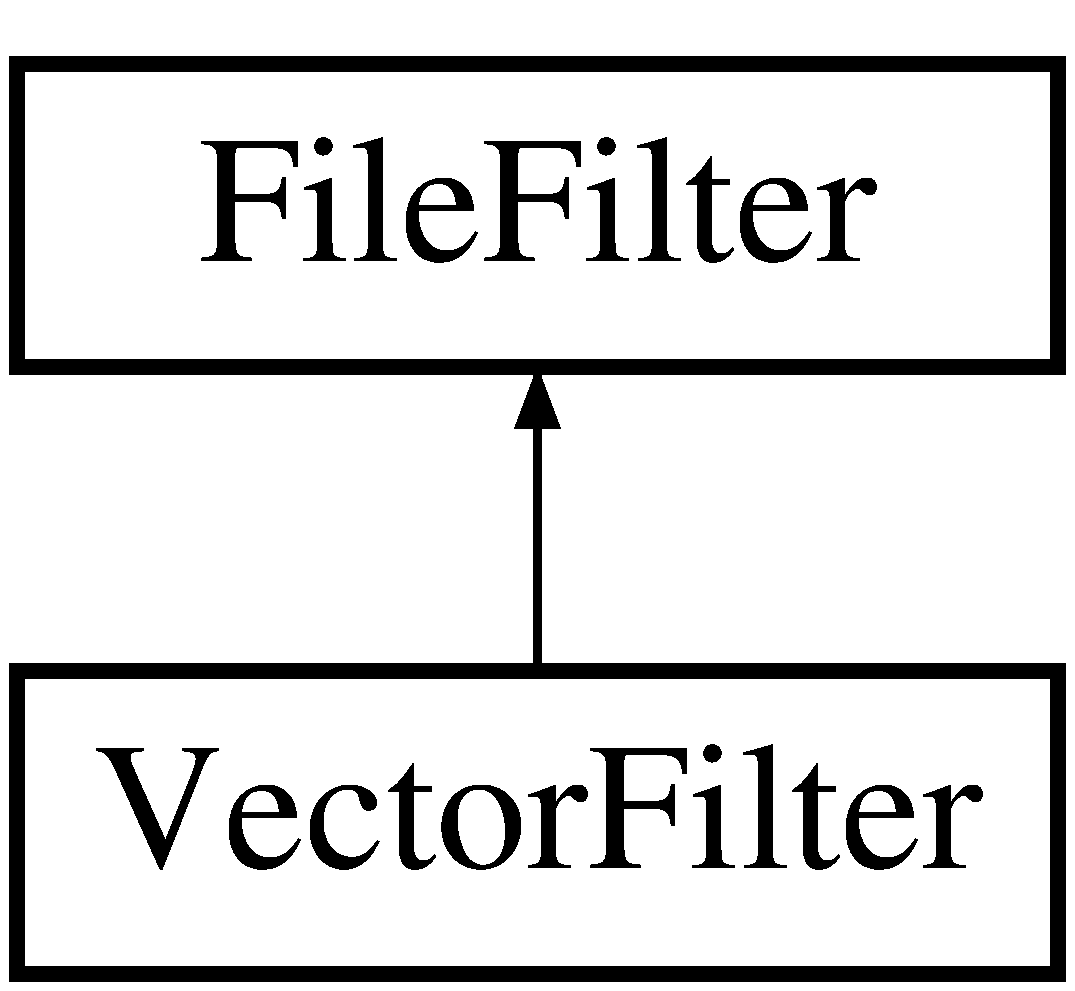
\includegraphics[height=2.000000cm]{class_vector_filter}
\end{center}
\end{figure}
\subsection*{Public Member Functions}
\begin{DoxyCompactItemize}
\item 
\mbox{\Hypertarget{class_vector_filter_a40b658a4acb3b68040d275ff6086a45e}\label{class_vector_filter_a40b658a4acb3b68040d275ff6086a45e}} 
boolean {\bfseries accept} (File f)
\item 
\mbox{\Hypertarget{class_vector_filter_abbdc1f2d0534ee36d137a34916f4bf29}\label{class_vector_filter_abbdc1f2d0534ee36d137a34916f4bf29}} 
String {\bfseries get\+Description} ()
\end{DoxyCompactItemize}


\subsection{Detailed Description}
Filter for J\+File\+Filter use \hyperlink{class_utils}{Utils} class \begin{DoxyAuthor}{Author}
Maciej Stosio 
\end{DoxyAuthor}
\begin{DoxyVersion}{Version}
1.\+0 
\end{DoxyVersion}


The documentation for this class was generated from the following file\+:\begin{DoxyCompactItemize}
\item 
Vector\+Filter.\+java\end{DoxyCompactItemize}

\hypertarget{class_window}{}\section{Window Class Reference}
\label{class_window}\index{Window@{Window}}
Inheritance diagram for Window\+:\begin{figure}[H]
\begin{center}
\leavevmode
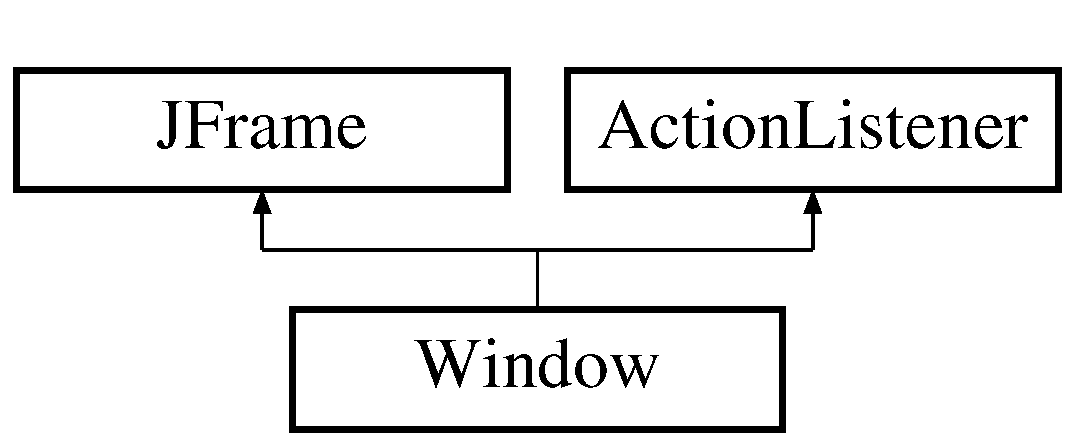
\includegraphics[height=2.000000cm]{class_window}
\end{center}
\end{figure}
\subsection*{Public Member Functions}
\begin{DoxyCompactItemize}
\item 
\hyperlink{class_window_ad0552903a3d5b009c0d882f9ad2571ff}{Window} ()
\item 
void \hyperlink{class_window_ab37b919572708606bcde411bf83d847a}{action\+Performed} (Action\+Event e)
\end{DoxyCompactItemize}
\subsection*{Static Public Attributes}
\begin{DoxyCompactItemize}
\item 
static Mode \hyperlink{class_window_add04f4568154de76f0e5359ab846a3cd}{mode}
\item 
static Color \hyperlink{class_window_ae9bd15543adc0d59f94321348c0ee8f7}{rgb} =Color.\+B\+L\+A\+CK
\item 
static J\+Panel \hyperlink{class_window_a212252a97adff44bb60a91a6c1a89975}{canvas}
\end{DoxyCompactItemize}


\subsection{Detailed Description}
Class handling window behavior. \begin{DoxyAuthor}{Author}
Maciej Stosio 
\end{DoxyAuthor}
\begin{DoxyVersion}{Version}
1.\+0 
\end{DoxyVersion}


\subsection{Constructor \& Destructor Documentation}
\mbox{\Hypertarget{class_window_ad0552903a3d5b009c0d882f9ad2571ff}\label{class_window_ad0552903a3d5b009c0d882f9ad2571ff}} 
\index{Window@{Window}!Window@{Window}}
\index{Window@{Window}!Window@{Window}}
\subsubsection{\texorpdfstring{Window()}{Window()}}
{\footnotesize\ttfamily Window.\+Window (\begin{DoxyParamCaption}{ }\end{DoxyParamCaption})}

Lunch main window. 

\subsection{Member Function Documentation}
\mbox{\Hypertarget{class_window_ab37b919572708606bcde411bf83d847a}\label{class_window_ab37b919572708606bcde411bf83d847a}} 
\index{Window@{Window}!action\+Performed@{action\+Performed}}
\index{action\+Performed@{action\+Performed}!Window@{Window}}
\subsubsection{\texorpdfstring{action\+Performed()}{actionPerformed()}}
{\footnotesize\ttfamily void Window.\+action\+Performed (\begin{DoxyParamCaption}\item[{Action\+Event}]{e }\end{DoxyParamCaption})}

Handle buttons\textquotesingle{} actions i.\+e change global mode, open info moda, save, open files, clear canvas. 

\subsection{Member Data Documentation}
\mbox{\Hypertarget{class_window_a212252a97adff44bb60a91a6c1a89975}\label{class_window_a212252a97adff44bb60a91a6c1a89975}} 
\index{Window@{Window}!canvas@{canvas}}
\index{canvas@{canvas}!Window@{Window}}
\subsubsection{\texorpdfstring{canvas}{canvas}}
{\footnotesize\ttfamily J\+Panel Window.\+canvas\hspace{0.3cm}{\ttfamily [static]}}

Cancvas \mbox{\Hypertarget{class_window_add04f4568154de76f0e5359ab846a3cd}\label{class_window_add04f4568154de76f0e5359ab846a3cd}} 
\index{Window@{Window}!mode@{mode}}
\index{mode@{mode}!Window@{Window}}
\subsubsection{\texorpdfstring{mode}{mode}}
{\footnotesize\ttfamily Mode Window.\+mode\hspace{0.3cm}{\ttfamily [static]}}

Selected global mode \mbox{\Hypertarget{class_window_ae9bd15543adc0d59f94321348c0ee8f7}\label{class_window_ae9bd15543adc0d59f94321348c0ee8f7}} 
\index{Window@{Window}!rgb@{rgb}}
\index{rgb@{rgb}!Window@{Window}}
\subsubsection{\texorpdfstring{rgb}{rgb}}
{\footnotesize\ttfamily Color Window.\+rgb =Color.\+B\+L\+A\+CK\hspace{0.3cm}{\ttfamily [static]}}

Global color 

The documentation for this class was generated from the following file\+:\begin{DoxyCompactItemize}
\item 
Window.\+java\end{DoxyCompactItemize}

%--- End generated contents ---

% Index
\backmatter
\newpage
\phantomsection
\clearemptydoublepage
\addcontentsline{toc}{chapter}{Index}
\printindex

\end{document}
